\documentclass[10pt,a4paper]{article}
\usepackage{ibaconnect}
\usepackage{float}
\docinfo{User Manual (Sprint 1)}{1.0}{19 Nov 2026}

\graphicspath{{figures/}}
% \screen{file}{width}{caption}
\newcommand{\screen}[3]{\begin{figure}[H]\centering\fbox{\includegraphics[width=#2\linewidth]{#1}}\caption{#3}\end{figure}}
\newcommand{\ui}[1]{\textbf{#1}}

\begin{document}
\makedoctitle

\section*{About this manual}
IBA Connect is a private network for IBA students and alumni. It helps you find the right person for a course, a project or career advice, ask them to connect, chat once they accept, and post what you need on the Need Board. This manual explains every Sprint 1 feature step by step. The screenshots are from the real application, taken with demo accounts that hold fictional data.

\textbf{What you need:} a recent version of Chrome, Edge, Firefox or Safari on a computer or phone. Students and staff use their IBA email (\texttt{@khi.iba.edu.pk}); alumni use a personal email and a code from the IBA Connect team, or an email the team has added to the alumni list.

\textbf{Menus:} on a computer the main menu is at the top of the page (\ui{Dashboard}, \ui{Directory}, \ui{Need Board}, \ui{Messages}, \ui{Requests}); on a phone it is a bar at the bottom of the screen. Your profile, settings and sign-out are in the \ui{account menu} (your initials or photo, top right). Numbers on \ui{Messages} and \ui{Requests} show unread messages and requests waiting for your answer.

\tableofcontents
\newpage

%-------------------------------------------------------------------------------------------
\section{Getting started}

\subsection{The home page}
Open the IBA Connect address in your browser. The home page explains what the network is for and offers \ui{Create account}, \ui{Sign in} and \ui{I am an alumnus}. If you are already signed in, you go straight to your dashboard.
\screen{landing}{0.85}{Home page}

\subsection{Create an account with your IBA email (US1.2)}
\begin{enumerate}
\item Click \ui{Create account}.
\item Enter your full name, your IBA email and a password. The password needs at least 8 characters with an uppercase letter, a lowercase letter, a number and a special character. Type it again to confirm.
\item Click \ui{Create account}. A page asks you to check your email.
\item Open the email from IBA Connect and click the verification link. You are taken to profile setup (section~\ref{sec:setup}).
\end{enumerate}
You cannot use the platform until your email is verified. If the email does not arrive, use \ui{Send a new link} on the \ui{Check your email} page.
\screen{register}{0.6}{Create an account}
\screen{verify-email}{0.6}{Check your email}

\subsection{Sign in with Microsoft (US1.1)}
If your IBA Microsoft account is enabled for IBA Connect, click \ui{Sign in with Microsoft (IBA)} on the sign-in page and sign in as you do for other IBA services. Only accounts on the IBA domain are accepted; any other Microsoft account is refused and no IBA Connect account is created. The first time, you are taken to profile setup.

\subsection{Sign in}
Click \ui{Sign in}, enter your email and password and click \ui{Sign in}. After too many wrong attempts you are asked to wait a few minutes before trying again.
\screen{sign-in}{0.6}{Sign in}

\subsection{Forgotten password (US1.3)}
\begin{enumerate}
\item On the sign-in page click \ui{Forgot password?}.
\item Enter your email and click \ui{Send reset link}.
\item Open the email and click the link, then choose a new password and confirm it.
\end{enumerate}
\screen{forgot-password}{0.6}{Forgot password}

\subsection{Alumni verification (US1.4)}
Alumni no longer have an IBA mailbox, so they register with a personal email.
\begin{enumerate}
\item On the home page click \ui{I am an alumnus}.
\item Choose how to verify: \ui{I have a code} (a code such as \texttt{IBA-7KQ2-M9XD} from the IBA Connect team) or \ui{My email is on the alumni list} (your personal email is already on the university's alumni list).
\item Enter your name, personal email, password and, if you chose a code, the code. Click \ui{Verify and create account}.
\item Confirm your email from the message you receive, then sign in.
\end{enumerate}
A code works once. Codes that are wrong, expired, revoked or already used are refused.
\screen{verify-alumni}{0.6}{Alumni verification}

%-------------------------------------------------------------------------------------------
\section{Your profile}

\subsection{Profile setup (US1.5)}\label{sec:setup}
The first time you sign in you are asked to set up your profile. Members only appear in the directory once their profile is finished.
\begin{enumerate}
\item Fill in your full name, batch (year of intake), programme, department and, if you are a current student, your semester.
\item Write a short bio (up to 500 characters) about what you study, work on or can help with.
\item Add at least one skill (up to 15). Start typing to pick from suggestions or add your own.
\item Choose the courses you have taken from the course list.
\item Click \ui{Finish setup}. Your dashboard opens.
\end{enumerate}
\screen{profile-setup}{0.75}{Profile setup}

\subsection{View and edit your profile (US1.6)}
Open the account menu and choose \ui{My profile} to see your profile as other members see it. Click \ui{Edit profile} to change any field, then \ui{Save changes}. Changes show at once on your profile and in directory search.
\screen{profile}{0.8}{Your profile}
\screen{profile-edit}{0.8}{Edit profile}

\subsection{Profile photo (US1.6)}
On \ui{Edit profile}, click \ui{Upload photo} (or \ui{Change photo}) and choose a PNG, JPEG or WebP image up to 2 MB. Other file types are refused. Click \ui{Remove} to go back to your initials.

\subsection{Alumni: field and company (US1.7)}
Alumni have two extra fields on their profile: the \ui{Field} they work in and their \ui{Company or organisation}. Both are shown on the profile and can be used as directory filters.
\screen{alumnus-profile}{0.8}{An alumnus profile with field and company}

\subsection{Available to advise (US1.8)}
If you are happy to help others with courses you have taken:
\begin{enumerate}
\item At the bottom of \ui{Edit profile}, in the \ui{Available to advise} card, switch on \ui{I am available to advise}.
\item Tick at least one of your courses that you can advise on. Without a course the setting cannot be saved.
\item Click \ui{Save}. An \ui{advise} badge appears on your profile and directory card, and you show up when someone filters by that course and \ui{Available to advise}.
\end{enumerate}
Turn the switch off to remove the badge.
\screen{advising}{0.8}{Available to advise}

%-------------------------------------------------------------------------------------------
\section{Dashboard (FR1.7)}
The dashboard is the first page after sign-in. It shows the number of requests waiting for your answer, your unread messages, your open Need Board posts and your connections. Each tile and list links to the full page, and the shortcuts reach every main screen in one or two clicks.
\screen{dashboard}{0.9}{Dashboard}

%-------------------------------------------------------------------------------------------
\section{Finding people}

\subsection{Browse the directory (US2.1)}
Click \ui{Directory} to see verified members, 18 per page. Each card shows the member's name, programme, batch, skills and any advising badge, with a link to their profile. Contact details are never shown in the directory.
\screen{directory}{0.9}{Directory}

\subsection{Search (US2.2)}
Type in the search box at the top of the directory and press Enter. The search looks at names, skills and course codes and titles; every word you type must match. If nobody matches, you see \ui{No members found} with a link to clear the search and filters.
\screen{directory-search}{0.9}{Searching for a skill}

\subsection{Filters (US2.3--US2.5)}
Use the filter panel (on a phone, tap \ui{Filter}) to narrow the list. Filters are listed in priority order: course, skill, available to advise, batch, department and programme. Alumni filters (field and company) show only alumni. Filters can be combined; each active filter appears as a chip you can remove, and \ui{Clear all} removes them all.
\begin{itemize}
\item \textbf{Find an adviser for a course:} choose the course and tick \ui{Available to advise}.
\item \textbf{Find alumni in a field:} choose the field, for example Banking \& Finance, or type a company.
\end{itemize}
\screen{directory-advise}{0.9}{Advisers for CSE341}
\screen{directory-alumni}{0.9}{Alumni in Banking \& Finance}

\subsection{Member profiles (US2.6)}
Click a card to open the member's profile: name, batch, programme, department, semester, bio, skills, courses and advising badge. Their email is shown only after they accept your connection request.
\screen{member-profile}{0.85}{A member's profile}

%-------------------------------------------------------------------------------------------
\section{Connections and messages}

\subsection{Send a connection request (US3.1, US3.2)}
\begin{enumerate}
\item Open the member's profile and click \ui{Connect}.
\item Write a short note saying why you are reaching out (up to 300 characters).
\item Click \ui{Send request}. The button changes to \ui{Request sent}.
\end{enumerate}
The member gets an email and sees the request under \ui{Requests}. You can send about ten requests a day. If someone declines, you have to wait a few days before asking them again.

\subsection{Answer requests and the requests inbox (US3.3, US3.4)}
Click \ui{Requests}. The page has three tabs: \ui{Incoming} (waiting for your answer), \ui{Outgoing} (requests you sent, with their status) and \ui{Accepted} (your connections). Each request shows the person, their note and, if it came from the Need Board, the post. Click \ui{Accept} to connect or \ui{Decline} to say no. Only accepted connections can chat.
\screen{requests-incoming}{0.85}{Incoming requests}
\screen{requests-accepted}{0.85}{Accepted connections}

\subsection{Chat (US3.5, US3.6)}
Click \ui{Messages} to see your chats, newest first, with a badge for unread messages. Open a chat, type a message (up to 2,000 characters) and press \ui{Send}. New messages from the other person appear within a few seconds without reloading. Opening a chat marks its messages as read and clears the badge.
\screen{messages}{0.85}{Chats}
\screen{chat}{0.85}{A conversation}

\subsection{Contact details (US3.7)}
When a request is accepted, both members can see each other's email on the profile and in the \ui{Accepted} tab. Before that, no email is shown anywhere.

\subsection{Block a member (FR3.7)}
On a member's profile open the \ui{More actions} menu (\ldots) and choose \ui{Block}. A blocked member cannot send you requests or messages, and you cannot contact them. Unblock them under \ui{Settings} $\rightarrow$ \ui{Blocked members}.

%-------------------------------------------------------------------------------------------
\section{Need Board}

\subsection{Browse the board (US4.2)}
Click \ui{Need Board} to see open posts from other members: study partners, project teammates, course advice and career advice. Filter by type, course or department, or search the text. Closed and expired posts are never listed.
\screen{board}{0.9}{Need Board}

\subsection{Post a need (US4.1)}
\begin{enumerate}
\item Click \ui{Post a need} (on the board or the dashboard).
\item Choose the type, write a title and the details.
\item Optionally tag a course or a department (one or the other).
\item Click \ui{Publish}. The post stays open for 14 days.
\end{enumerate}
\screen{board-new}{0.75}{Post a need}

\subsection{Respond to a post (US4.3)}
Open a post and click \ui{Respond}, write a short reply and send it. This sends the author a connection request linked to the post, so the same daily limit applies. You cannot respond to your own post.

\subsection{Your posts: edit, close and expiry (US4.4, US4.5, FR4.5)}
Open \ui{Need Board} $\rightarrow$ \ui{My posts} to see your posts with their state (open, closed or expired) and the number of responses. Open a post to see who responded. While a post is open you can \ui{Edit} its title, details and tag, or \ui{Close} it early when you have found someone. After 14 days a post expires by itself. Closed and expired posts leave the board, but you can still see their responses.
\screen{my-posts}{0.85}{My posts}
\screen{my-post-detail}{0.85}{A post with its responses}

%-------------------------------------------------------------------------------------------
\section{Settings and your account}

\subsection{Change your password (US1.3)}
Open the account menu and choose \ui{Settings}. Under \ui{Password}, enter your current password and the new one twice, then click \ui{Change password}. Other devices are signed out.
\screen{settings}{0.85}{Settings}

\subsection{Sign out and session expiry (FR1.6)}
Choose \ui{Sign out} in the account menu. For your safety you are also signed out automatically after a long period without activity; just sign in again.

\subsection{Deactivate or delete your account (FR1.8)}
Under \ui{Settings} $\rightarrow$ \ui{Account}:
\begin{itemize}
\item \ui{Deactivate} hides your profile from the directory and signs you out. Sign in again to reactivate.
\item \ui{Delete account} removes your account for good. Type \texttt{DELETE} to confirm. Your messages stay in other members' chats but show \emph{Deleted member} instead of your name. Choosing \ui{Cancel} changes nothing.
\end{itemize}
\screen{account-actions}{0.85}{Deactivate or delete}

%-------------------------------------------------------------------------------------------
\section{For administrators}
Administrators see \ui{Admin panel} in the account menu. Other members cannot open it.
\screen{admin}{0.85}{Admin panel}

\subsection{Alumni codes and the alumni list (FR1.9)}
Open \ui{Alumni verification}.
\begin{itemize}
\item \textbf{Issue a code:} choose how long it is valid (or no expiry), add an optional note such as the alumnus's name, and click \ui{New code}. Copy the code and send it to the alumnus.
\item \textbf{Expire or revoke a code} that has not been used yet. Each code shows its status: active, claimed, expired or revoked.
\item \textbf{Upload the alumni list:} choose a CSV file whose first row names the columns (\texttt{email} is required, \texttt{name} and \texttt{batch} are optional). Emails already on the list are skipped, and rows with errors are reported.
\end{itemize}
Every change is recorded in the audit log.
\screen{admin-alumni}{0.85}{Alumni codes and alumni list}

\subsection{Course list (FR1.10)}
Open \ui{Course list} to add a course (code, title, department), edit one, or retire one. A retired course is no longer offered in pickers but stays on the profiles that already list it. Course codes must be unique.
\screen{admin-courses}{0.85}{Course list}

%-------------------------------------------------------------------------------------------
\section{Using IBA Connect on a phone}
Every page works at phone width. The main menu moves to a bar at the bottom of the screen, and the directory filters open from the \ui{Filter} button.
\begin{figure}[H]\centering
\fbox{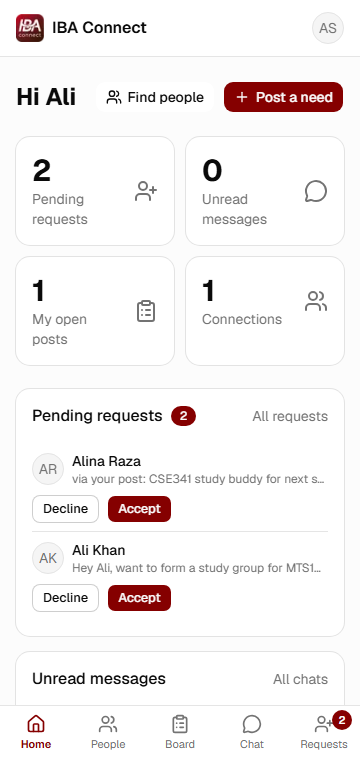
\includegraphics[width=0.3\linewidth]{mobile-dashboard}}\hspace{1cm}\fbox{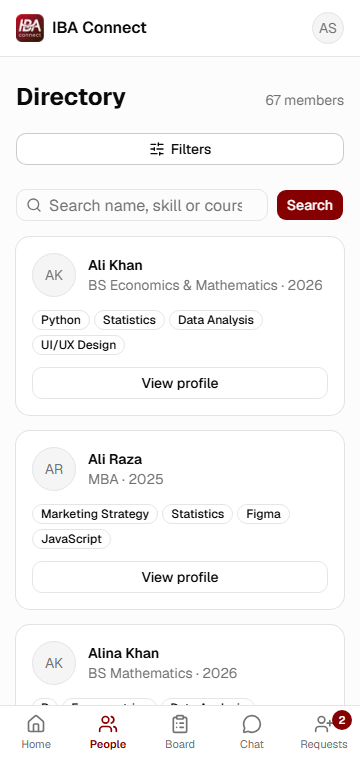
\includegraphics[width=0.3\linewidth]{mobile-directory}}
\caption{Dashboard and directory on a phone}
\end{figure}

\section{Help and privacy}
\begin{itemize}
\item Your email is only shown to members who accepted your request, and to you.
\item Only verified IBA students, staff and alumni can see the directory.
\item For help with alumni codes or a suspended account, contact the IBA Connect team.
\end{itemize}

\end{document}
